\documentclass{beamer}
\usepackage[uofc]{nathanngo}
\usepackage[style=apa,backend=biber]{biblatex}
\usepackage{animate,randomwalk,pgfplots}
\usepackage{pgfplotstable}
\pgfplotsset{compat=1.18}
\addbibresource{references.bib}

\title{PHYS598}
\subtitle{Investigating Two-Step Perfect Quantum State Transfer in Quantum Walks}
\author{Nathan Ngo\\Supervisor: David Feder}
\institute{University of Calgary}
\date{April 4, 2025}

\begin{document}

\maketitle

\section{Classical Random Walk}
\begin{frame}{What is it?}
    \begin{itemize}
        \item  Moves step by step in a certain space, according to specific probabilistic rules
    \end{itemize}
\end{frame}
\begin{frame}{Discrete-Time Classical Random Walk}
    \begin{itemize}
        \item \textbf Moves at specific, regular intervals
    \end{itemize}
    \begin{displaymath}
        P(x,n+1)=\frac{1}{2}P(x-1,n)+\frac{1}{2}P(x+1,n)
    \end{displaymath}
    \begin{center}
        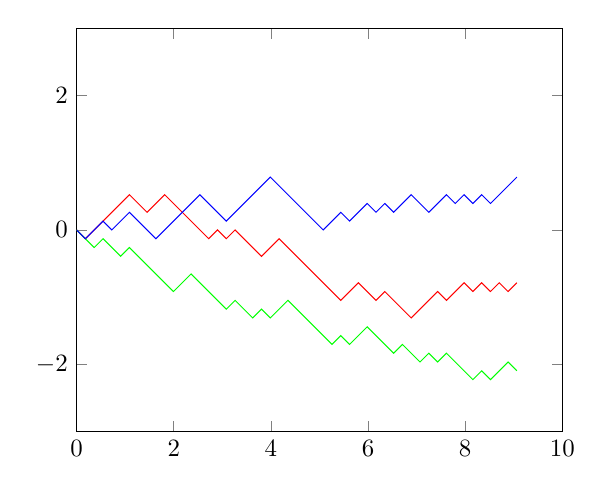
\begin{tikzpicture}[scale=0.9]
        \begin{axis}[
        xmin=0, xmax=10,
        ymin=-3, ymax=3,
        ]
        \draw[red] (0,0) \foreach \i in {1,...,50}{ -- ++({(2*random(0,1)-1)*45}:5pt) };
        \draw[green] (0,0) \foreach \i in {1,...,50}{ -- ++({(2*random(0,1)-1)*45}:5pt) };
        \draw[blue] (0,0) \foreach \i in {1,...,50}{ -- ++({(2*random(0,1)-1)*45}:5pt) };
        \end{axis}
        \end{tikzpicture}
    \end{center}
\end{frame}
\begin{frame}{Continuous-Time Classical Random Walk}
    \begin{itemize}
        \item \textbf Moves at any time, not just at fixed intervals
    \end{itemize}
    \begin{displaymath}
        \frac{\partial P(x,t)}{\partial t}=D\frac{\partial^2P(x,t)}{\partial x^2}
    \end{displaymath}
    \begin{center}
        \begin{tikzpicture}[scale=0.9]
        \begin{axis}[
        xmin=0, xmax=10,
        ymin=-3, ymax=3,
        ]
        \draw[red] (0,0) \foreach \i in {1,...,100}{ -- ++({(2*random(0,1)-1)*10}:2pt) };
        \draw[green] (0,0) \foreach \i in {1,...,100}{ -- ++({(2*random(0,1)-1)*10}:2pt) };
        \draw[blue] (0,0) \foreach \i in {1,...,100}{ -- ++({(2*random(0,1)-1)*10}:2pt) };
        \end{axis}
        \end{tikzpicture}
    \end{center}
\end{frame}
\section{Quantum Walk}
\begin{frame}{What is it?}
    \begin{itemize}
        \item In quantum mechanics, particles can exist in superpositions
        \item Particles can be in a superposition of several positions simultaneously
    \end{itemize}
\end{frame}
\begin{frame}{Discrete-Time Quantum Walk}
    \begin{itemize}
        \item \textbf Moves at specific, regular intervals
    \end{itemize}
    \begin{center}
        
\includegraphics[scale=0.5]{PHYS598 Final Presentation/discrete.png}
    \end{center}
\end{frame}
\begin{frame}{Continuous-Time Quantum Walk}
    \begin{itemize}
        \item Evolves smoothly rather than in discrete steps
    \end{itemize}
    \begin{displaymath}
        i\hbar\frac{\partial\psi(x,t)}{\partial t}=-\frac{\hbar^2}{2m}\frac{\partial^2\psi(x,t)}{\partial x^2}
    \end{displaymath}
    \begin{center}
        
\includegraphics[scale=0.5]{PHYS598 Final Presentation/quantum-1.png}
    \end{center}
\end{frame}
\section{Graph Theory}
\begin{frame}{What is it?}
    \begin{itemize}
        \item Mathematical study of structures called graphs: composed of nodes (vertices) and edges (connections)
        \item Graphs model relationships between objects in a variety of fields
    \end{itemize}
    \begin{center}
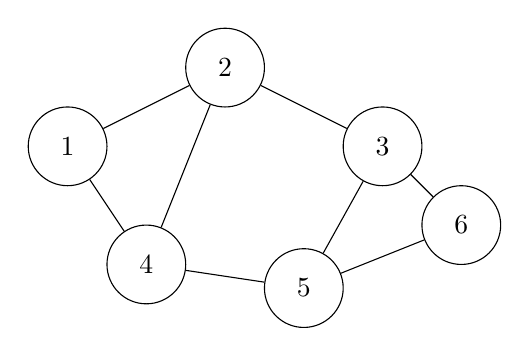
\begin{tikzpicture}
    % Draw nodes
    \node[circle, draw, fill=white, minimum size=1cm] (A) at (0,0) {1};
    \node[circle, draw, fill=white, minimum size=1cm] (B) at (2,1) {2};
    \node[circle, draw, fill=white, minimum size=1cm] (C) at (4,0) {3};
    \node[circle, draw, fill=white, minimum size=1cm] (D) at (1,-1.5) {4};
    \node[circle, draw, fill=white, minimum size=1cm] (E) at (3,-1.8) {5};
    \node[circle, draw, fill=white, minimum size=1cm] (F) at (5,-1) {6};

    % Draw connections (messy/random)
    \draw[-] (A) -- (B) node[midway, above left] {};
    \draw[-] (B) -- (C) node[midway, above] {};
    \draw[-] (C) -- (F) node[midway, right] {};
    \draw[-] (B) -- (D) node[midway, left] {};
    \draw[-] (D) -- (E) node[midway, below] {};
    \draw[-] (E) -- (F) node[midway, below right] {};
    \draw[-] (A) -- (D) node[midway, left] {};
    \draw[-] (C) -- (E) node[midway, below] {};

\end{tikzpicture}
\end{center}

\end{frame}

\begin{frame}{How is a Quantum Problem also a Graph Problem?}
    \begin{center}
        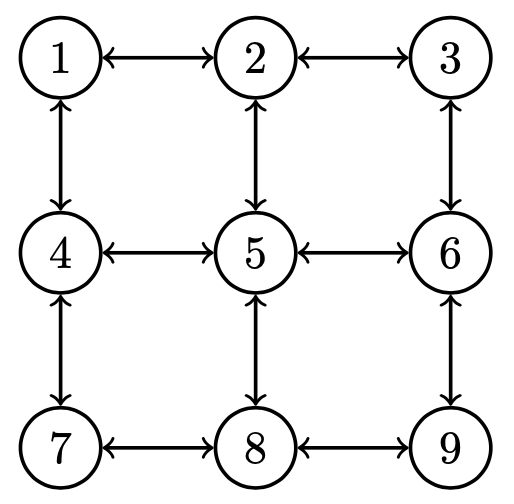
\includegraphics[scale=0.5]{2D Path.png}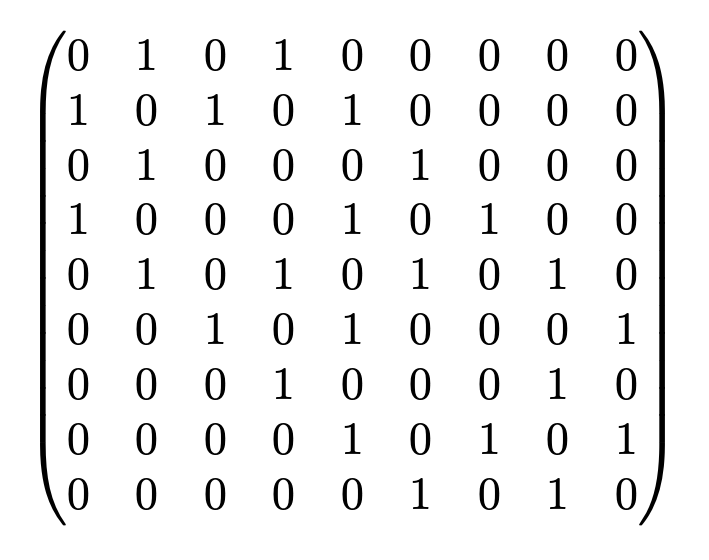
\includegraphics[scale=0.45]{Adjacency Matrix.png}
    \end{center}
\end{frame}
\section{One-Step Perfect Quantum State Transfer (PST)}
\begin{frame}{What is it?}
    \begin{itemize}
        \item An exact transfer of a quantum state from node $A$ to node $B$ with a perfect fidelity\footfullcite{BabukhinD.V.2022Teoq}
        \item A promising tool for quantum information science\footnotemark[3]
        \item A rare phenomenon, hard to find new candidates\footfullcite{COUTINHO2022155}
    \end{itemize}
    \begin{center}
    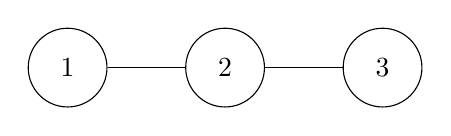
\begin{tikzpicture}
    % Draw nodes
    \node[circle, draw, fill=white, minimum size=1cm] (1) at (0,0) {1};
    \node[circle, draw, fill=white, minimum size=1cm] (2) at (2,0) {2};
    \node[circle, draw, fill=white, minimum size=1cm] (3) at (4,0) {3};
    
    % Draw connections
    \draw[-] (1) -- (2);
    \draw[-] (2) -- (3);
    
    % Labels
    \node[below] at (1) {};
    \node[below] at (2) {};
    \node[below] at (3) {};
\end{tikzpicture}
\end{center}
\end{frame}
\section{Two-Step Perfect Quantum State Transfer (PST)}
\begin{frame}{Differences between One-Step and Two Step PST}
    \begin{itemize}
        \item Let the quantum state evolve on the initial graph configuration for a specified duration
        \item  Introduce a controlled modification to the graph structure
        \item Allow the system to evolve for a second period of time
    \end{itemize}
\end{frame}
\begin{frame}{Why do we care?}
    \begin{itemize}
        \item High flexibility
        \item Avoid decoherence
    \end{itemize}
\end{frame}
\section{Research Questions}
\begin{frame}{What is left to figure out?}
    \begin{itemize}
        \item Which graph structures support two-step PST?
        \item What are the conditions for two-step PST?
        \item How do edge weights and vertex configurations affect PST?
    \end{itemize}
\end{frame}
\begin{frame}{Graph Selection}
    \begin{itemize}
        \item P$_4$: \begin{center}
            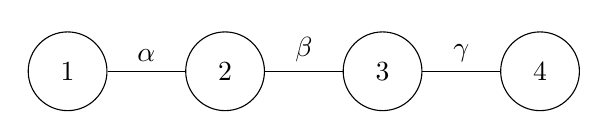
\begin{tikzpicture}
            % Draw nodes
            \node[circle, draw, fill=white, minimum size=1cm] (1) at (0,0) {1};
            \node[circle, draw, fill=white, minimum size=1cm] (2) at (2,0) {2};
            \node[circle, draw, fill=white, minimum size=1cm] (3) at (4,0) {3};
            \node[circle, draw, fill=white, minimum size=1cm] (4) at (6,0) {4};
            
            % Draw connections
            \draw[-] (1) -- (2) node[midway, above] {$\alpha$};
            \draw[-] (2) -- (3) node[midway, above] {$\beta$};
            \draw[-] (3) -- (4) node[midway, above] {$\gamma$};
            
            % Labels
            \node[below] at (1) {};
            \node[below] at (2) {};
            \node[below] at (3) {};
            \node[below] at (4) {};
        \end{tikzpicture}
        \end{center}
        \item C$_3$: \begin{center}
            \begin{tikzpicture}
            % Draw nodes
            \node[circle, draw, fill=white, minimum size=1cm] (1) at (0,1.5) {1};
            \node[circle, draw, fill=white, minimum size=1cm] (2) at (2.6,-1.5) {2};
            \node[circle, draw, fill=white, minimum size=1cm] (3) at (-2.6,-1.5) {3};
            
            % Draw connections
            \draw[-] (1) -- (2) node[midway, right] {$\alpha$};
            \draw[-] (2) -- (3) node[midway, below] {$\beta$};
            \draw[-] (3) -- (1) node[midway, left] {$\gamma$};
            
            % Labels
            \node[below] at (1) {};
            \node[below] at (2) {};
            \node[below] at (3) {};
        \end{tikzpicture}
        \end{center}
        where $\alpha,\beta,\gamma\in\mathbb{R}$.
    \end{itemize}
\end{frame}
\begin{frame}{Why P$_4$?}
    \begin{itemize}
        \item Two known cases of PST from node 1 to 4
        \item Motivates search for a broader family with similar behavior
    \end{itemize}
    \begin{center}
            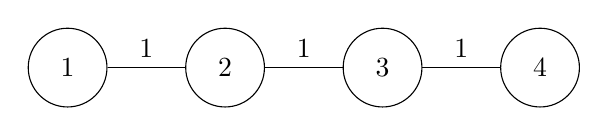
\begin{tikzpicture}
            % Draw nodes
            \node[circle, draw, fill=white, minimum size=1cm] (1) at (0,0) {1};
            \node[circle, draw, fill=white, minimum size=1cm] (2) at (2,0) {2};
            \node[circle, draw, fill=white, minimum size=1cm] (3) at (4,0) {3};
            \node[circle, draw, fill=white, minimum size=1cm] (4) at (6,0) {4};
            
            % Draw connections
            \draw[-] (1) -- (2) node[midway, above] {$1$};
            \draw[-] (2) -- (3) node[midway, above] {$1$};
            \draw[-] (3) -- (4) node[midway, above] {$1$};
            
            % Labels
            \node[below] at (1) {};
            \node[below] at (2) {};
            \node[below] at (3) {};
            \node[below] at (4) {};
        \end{tikzpicture}
    \end{center}
        \begin{center}
            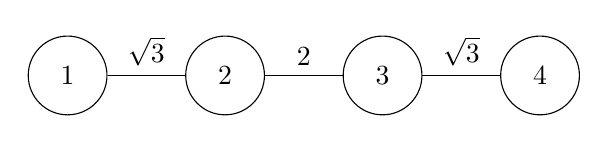
\begin{tikzpicture}
            % Draw nodes
            \node[circle, draw, fill=white, minimum size=1cm] (1) at (0,0) {1};
            \node[circle, draw, fill=white, minimum size=1cm] (2) at (2,0) {2};
            \node[circle, draw, fill=white, minimum size=1cm] (3) at (4,0) {3};
            \node[circle, draw, fill=white, minimum size=1cm] (4) at (6,0) {4};
            
            % Draw connections
            \draw[-] (1) -- (2) node[midway, above] {$\sqrt{3}$};
            \draw[-] (2) -- (3) node[midway, above] {$2$};
            \draw[-] (3) -- (4) node[midway, above] {$\sqrt{3}$};
            
            % Labels
            \node[below] at (1) {};
            \node[below] at (2) {};
            \node[below] at (3) {};
            \node[below] at (4) {};
        \end{tikzpicture}
        \end{center}
        \begin{center}
            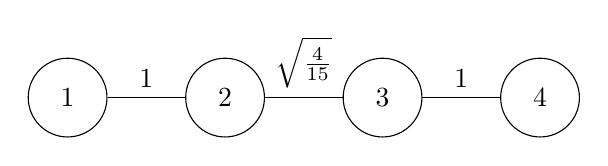
\begin{tikzpicture}
            % Draw nodes
            \node[circle, draw, fill=white, minimum size=1cm] (1) at (0,0) {1};
            \node[circle, draw, fill=white, minimum size=1cm] (2) at (2,0) {2};
            \node[circle, draw, fill=white, minimum size=1cm] (3) at (4,0) {3};
            \node[circle, draw, fill=white, minimum size=1cm] (4) at (6,0) {4};
            
            % Draw connections
            \draw[-] (1) -- (2) node[midway, above] {$1$};
            \draw[-] (2) -- (3) node[midway, above] {$\sqrt{\frac{4}{15}}$};
            \draw[-] (3) -- (4) node[midway, above] {$1$};
            
            % Labels
            \node[below] at (1) {};
            \node[below] at (2) {};
            \node[below] at (3) {};
            \node[below] at (4) {};
        \end{tikzpicture}
    \end{center}
\end{frame}
\begin{frame}{Why C$_3$?}
    \begin{itemize}
        \item No known PST cases with real edge weights — all known cases use imaginary weights
    \end{itemize}
    \begin{center}
        \begin{tikzpicture}
        % Draw nodes
        \node[circle, draw, fill=white, minimum size=1cm] (1) at (0,1.5) {1};
        \node[circle, draw, fill=white, minimum size=1cm] (2) at (2.6,-1.5) {2};
        \node[circle, draw, fill=white, minimum size=1cm] (3) at (-2.6,-1.5) {3};
        
        % Draw connections
        \draw[-] (1) -- (2) node[midway, right] {$\alpha$};
        \draw[-] (2) -- (3) node[midway, below] {$\beta$};
        \draw[-] (3) -- (1) node[midway, left] {$\gamma$};
        
        % Labels
        \node[below] at (1) {};
        \node[below] at (2) {};
        \node[below] at (3) {};
    \end{tikzpicture}
    \end{center}
\end{frame}
\section{Methodology}
\begin{frame}{How would I do it?}
    \begin{enumerate}
        \item Optimizer implementation
        \item Identification of mathematical structures
        \item Analytical verification
        \item Pattern recognition
    \end{enumerate}
\end{frame}
\begin{frame}{Optimizer Implementation}
    \begin{itemize}
        \item Implemented in Python using TensorFlow
        \item Used Adam optimizer to maximize fidelity
        \item Variables: edge weights (before/after), and runtime (before/after adjustment)
        \item Output: Lists of irrational numbers
    \end{itemize}
    \begin{center}
        \begin{displaymath}
            \text{Fidelity}\leq0.999999999999
        \end{displaymath}
        \begin{tabular}{||c c c||}
            \hline
            Initial Edge Weights&Final Edge Weights&$t=t'$\\
            \hline
            [1.0, -2.2677868380760757, 1.0]&[-1.0, -2.2677868380760757, -1.0]&2.077831382\\
    
            [1.0, -2.2677868380760757, 1.0]&[-1.0, -2.2677868380760757, -1.0]&2.077831382\\
            \hline
            [1.0, -7.281358514018219, 1.0]&[-1.0, -7.281358514018219, -1.0]&5.824775131\\
            \hline
            [1.0, 0.1672484025560938, 1.0]&[-1.0, 0.1672484025560938, -1.0]&9.392512825\\
            \hline
        \end{tabular}
    \end{center}
\end{frame}
\begin{frame}{Identification of Mathematical Structures}
    \begin{displaymath}
        -2.2677868380760757\rightarrow-\frac{6}{\sqrt{7}}
    \end{displaymath}
    \begin{displaymath}
        2.077831382\rightarrow\frac{\sqrt{7}}{4}\pi
    \end{displaymath}
\end{frame}
\begin{frame}{Analytical Verification}
    \begin{itemize}
        \item Substitute guessed mathematical forms into Mathematica
        \item Verify if fidelity evaluates to exactly 1
        \item If not, repeat the last step
    \end{itemize}
\end{frame}
\begin{frame}{Pattern Recognition}
    \begin{itemize}
        \item Identify patterns in edge weights (before/after)
        \item Relate edge weights to corresponding runtimes
        \item Generalize to a broader family
    \end{itemize}
\end{frame}
\section{Results}
\begin{frame}{P$_4$: Two-Step PST from Node 1 to Node 4}
    \begin{figure}
        \centering
        \begin{tikzpicture}[scale=1.5]
            % Draw nodes
            \node[circle, draw, fill=white, minimum size=1cm] (1) at (0,0) {1};
            \node[circle, draw, fill=white, minimum size=1cm] (2) at (2,0) {2};
            \node[circle, draw, fill=white, minimum size=1cm] (3) at (4,0) {3};
            \node[circle, draw, fill=white, minimum size=1cm] (4) at (6,0) {4};
            
            % Draw connections
            \draw[-] (1) -- (2) node[midway, above] {$\gamma$};
            \draw[-] (2) -- (3) node[midway, above] {$\nicefrac{\alpha\gamma}{\sqrt{\beta}}$};
            \draw[-] (3) -- (4) node[midway, above] {$\gamma$};
        \end{tikzpicture}
        \begin{tikzpicture}[scale=1.5]
            % Draw nodes
            \node[circle, draw, fill=white, minimum size=1cm] (1) at (0,0) {1};
            \node[circle, draw, fill=white, minimum size=1cm] (2) at (2,0) {2};
            \node[circle, draw, fill=white, minimum size=1cm] (3) at (4,0) {3};
            \node[circle, draw, fill=white, minimum size=1cm] (4) at (6,0) {4};
            
            % Draw connections
            \draw[-] (1) -- (2) node[midway, above] {$-\gamma$};
            \draw[-] (2) -- (3) node[midway, above] {$\nicefrac{\alpha\gamma}{\sqrt{\beta}}$};
            \draw[-] (3) -- (4) node[midway, above] {$-\gamma$};
        \end{tikzpicture}
    \end{figure}
    \begin{align}
        \beta &= 7 + 8n = (5+p)(3 - p + 8m), \\
        \alpha &= 2 + 2p - 8m, \\
        &\text{where} \quad
        \begin{cases}
            n = 0,1,2,\dots, \\
            m = 0,1,2,\dots,n.
        \end{cases}\nonumber
    \end{align}
    If $p\in\mathbb{Z}$ and $\nicefrac{\alpha}{\sqrt{\beta}}$ is in its simplest form $\nicefrac{\alpha'}{\sqrt{\beta'}}$ where $\alpha',\beta'\in\mathbb{Z}$, then the shortest time needed to achieve perfect fidelity is $t = t' = \frac{\sqrt{\beta'} \pi}{4\gamma}$.
\end{frame}
\begin{frame}{Two-Step PST Revealed as One-Step PST}
    \begin{figure}
        \centering
        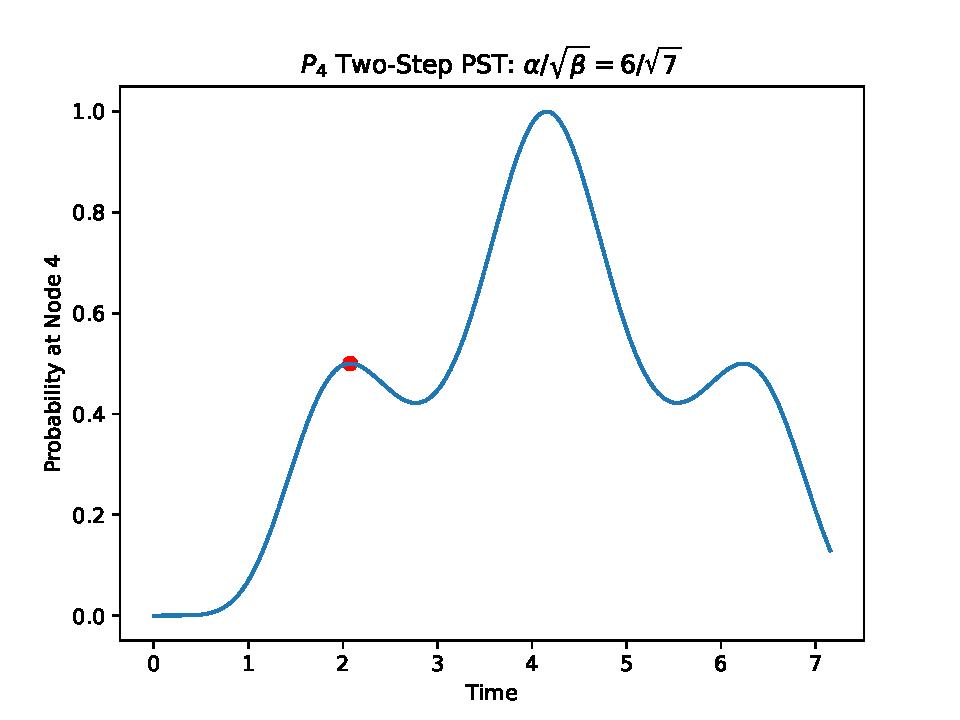
\includegraphics[width=0.49\linewidth]{graph 1.pdf}
        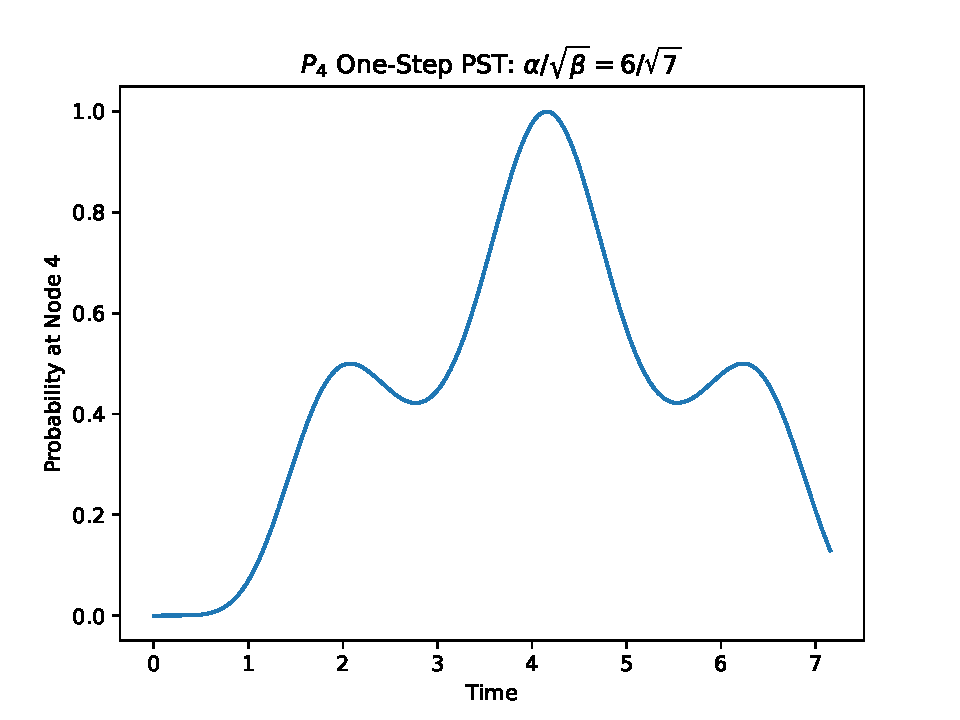
\includegraphics[width=0.49\linewidth]{graph 2.pdf}
    \end{figure}
\end{frame}
\begin{frame}{Two-Step PST Revealed as One-Step PST}
    \begin{itemize}
        \item Two-step PST family found to be realizable in a single step
        \item For P$_4$, adjusting edge weight at a probability peak has no effect on dynamics
        \item Verified in Mathematica as a new one-step PST family
    \end{itemize}
\end{frame}
\begin{frame}{C$_3$: Two Step PST from Node 1 to Node 2}
    \begin{center}
        \begin{tikzpicture}
        % Draw nodes
        \node[circle, draw, fill=white, minimum size=1cm] (1) at (0,1.5) {1};
        \node[circle, draw, fill=white, minimum size=1cm] (2) at (2.6,-1.5) {2};
        \node[circle, draw, fill=white, minimum size=1cm] (3) at (-2.6,-1.5) {3};
        
        % Draw connections
        \draw[-] (1) -- (2) node[midway, right] {$1$};
        \draw[-] (2) -- (3) node[midway, below] {$\beta$};
        \draw[-] (3) -- (1) node[midway, left] {$\beta$};
        
        % Labels
        \node[below] at (1) {};
        \node[below] at (2) {};
        \node[below] at (3) {};
    \end{tikzpicture}
        \begin{tikzpicture}
        % Draw nodes
        \node[circle, draw, fill=white, minimum size=1cm] (1) at (0,1.5) {1};
        \node[circle, draw, fill=white, minimum size=1cm] (2) at (2.6,-1.5) {2};
        \node[circle, draw, fill=white, minimum size=1cm] (3) at (-2.6,-1.5) {3};
        
        % Draw connections
        \draw[-] (1) -- (2) node[midway, right] {$1$};
        \draw[-] (2) -- (3) node[midway, below] {$\beta$};
        \draw[-] (3) -- (1) node[midway, left] {$-\beta$};
        
        % Labels
        \node[below] at (1) {};
        \node[below] at (2) {};
        \node[below] at (3) {};
    \end{tikzpicture}
    \end{center}
\end{frame}
\begin{frame}{Honourable Mentions}
    \begin{figure}
        \centering
        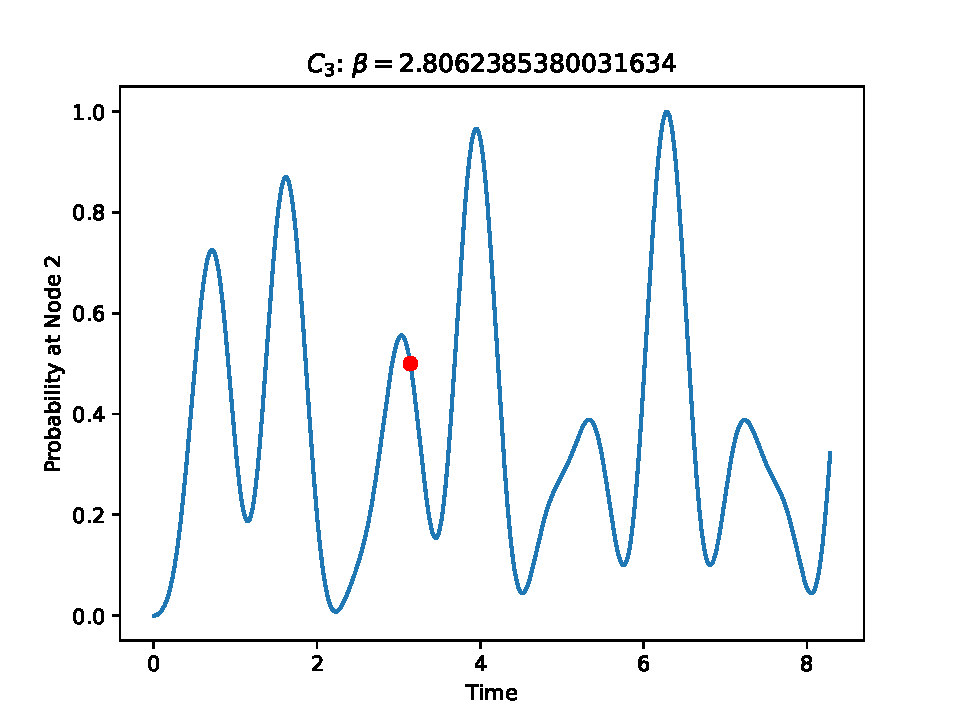
\includegraphics[width=0.49\textwidth]{c_3 (1).pdf}
        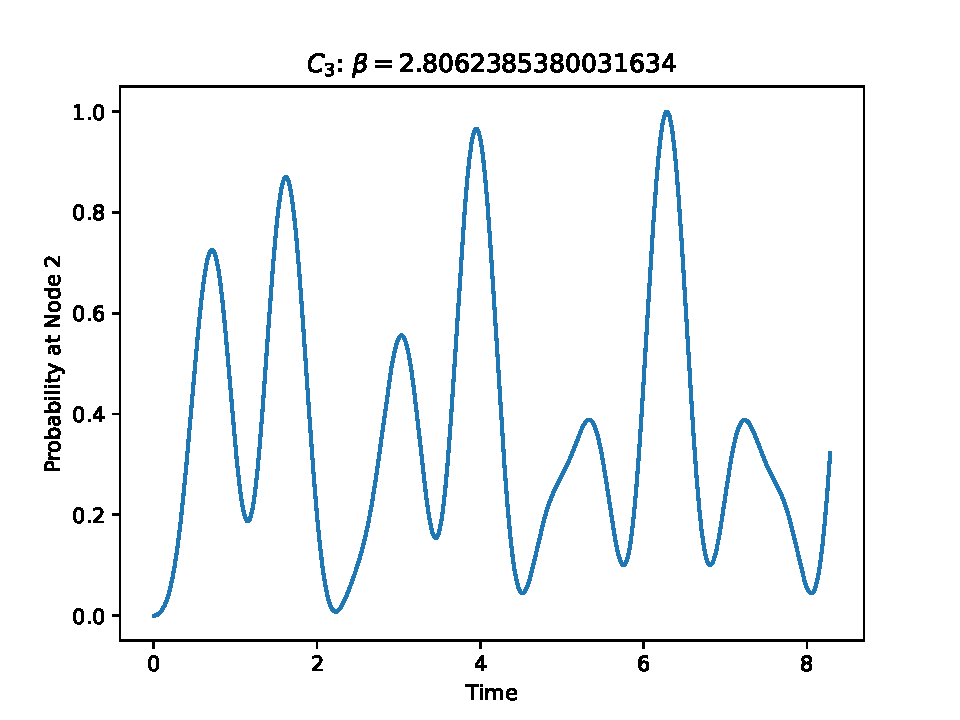
\includegraphics[width=0.49\textwidth]{c_3 (2).pdf}
    \end{figure}
    \begin{center}
        $\text{Fidelity}\geq0.999999999999$ at $t\approx2\pi$
    \end{center}
\end{frame}
\begin{frame}{Honourable Mentions}
    \begin{figure}
        \centering
        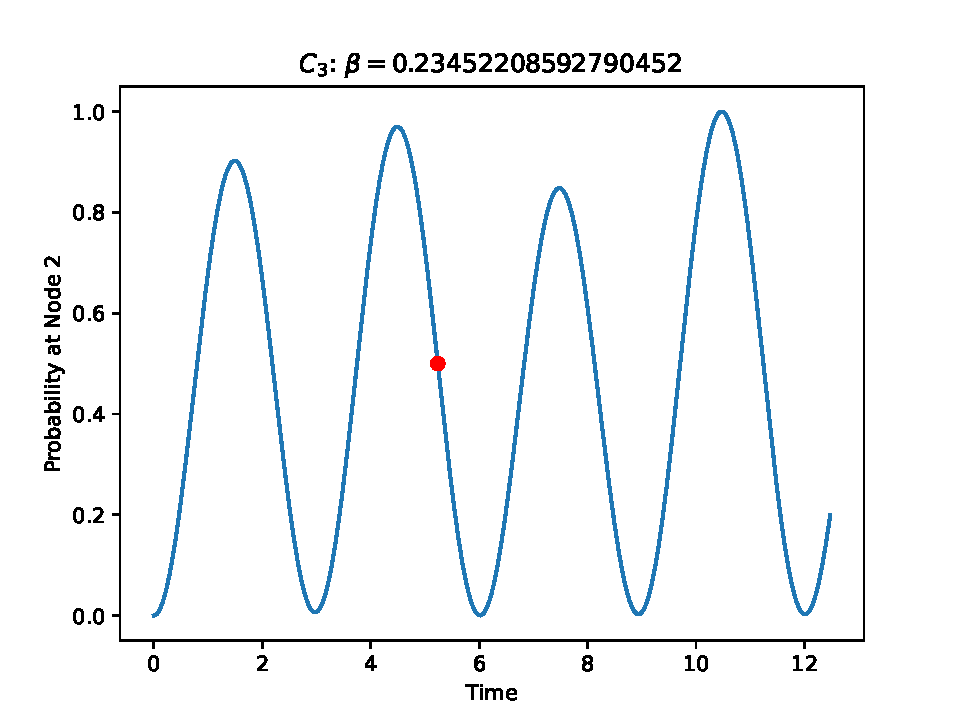
\includegraphics[width=0.49\textwidth]{c_3 (3).pdf}
        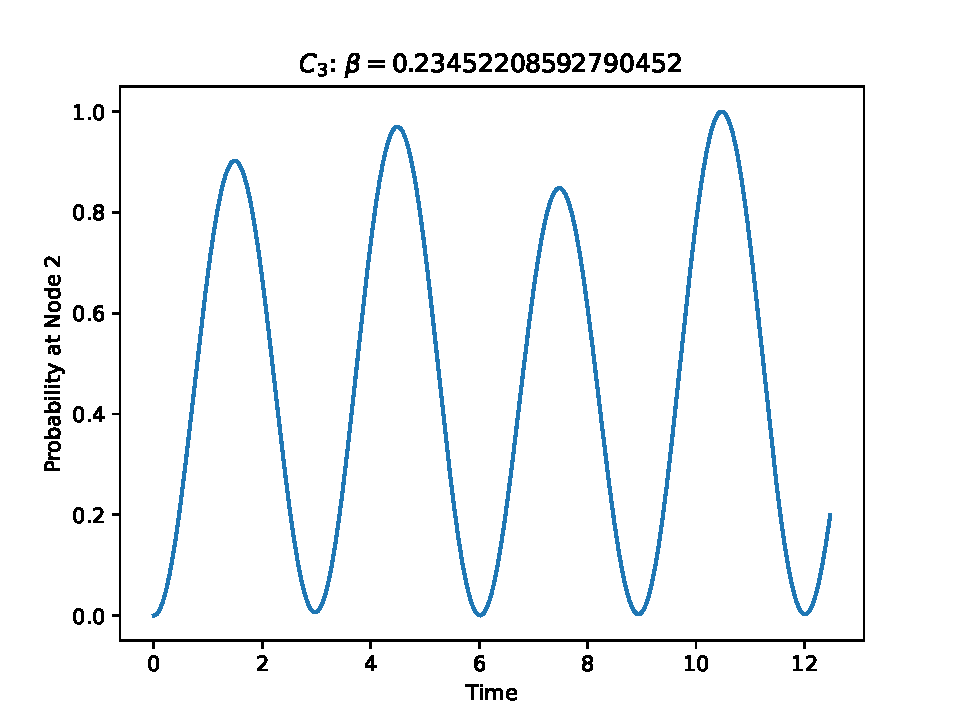
\includegraphics[width=0.49\textwidth]{c_3 (4).pdf}
    \end{figure}
    \begin{center}
        $\text{Fidelity}\geq0.999999999999$ at $t\approx\nicefrac{10\pi}{3}$
    \end{center}
\end{frame}
\begin{frame}{Honourable Mentions}
    \begin{figure}
        \centering
        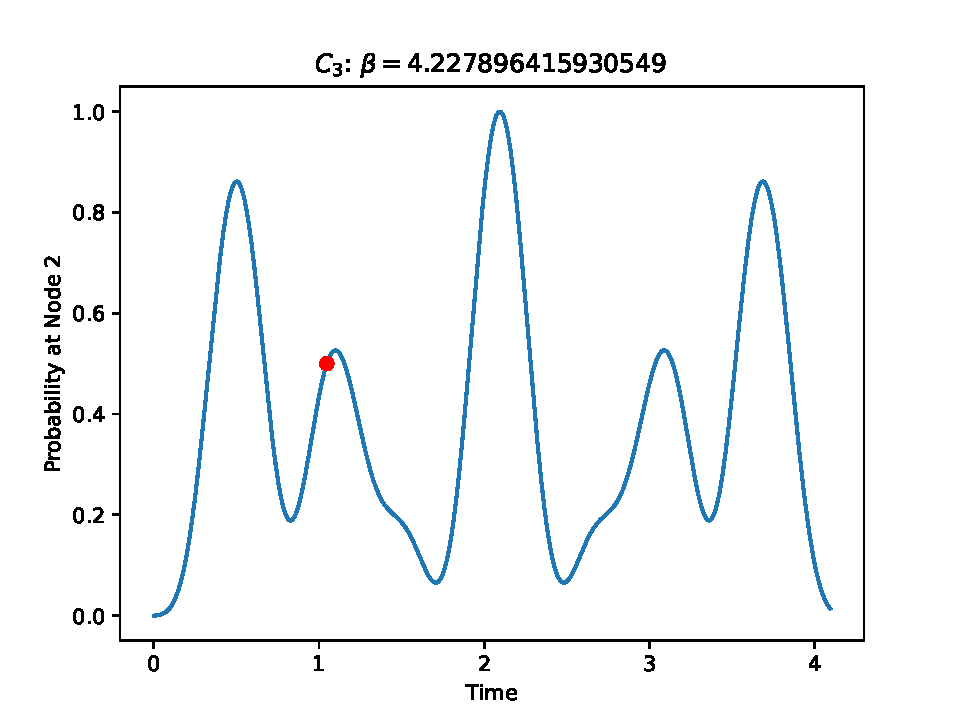
\includegraphics[width=0.49\textwidth]{c_3 (5).pdf}
        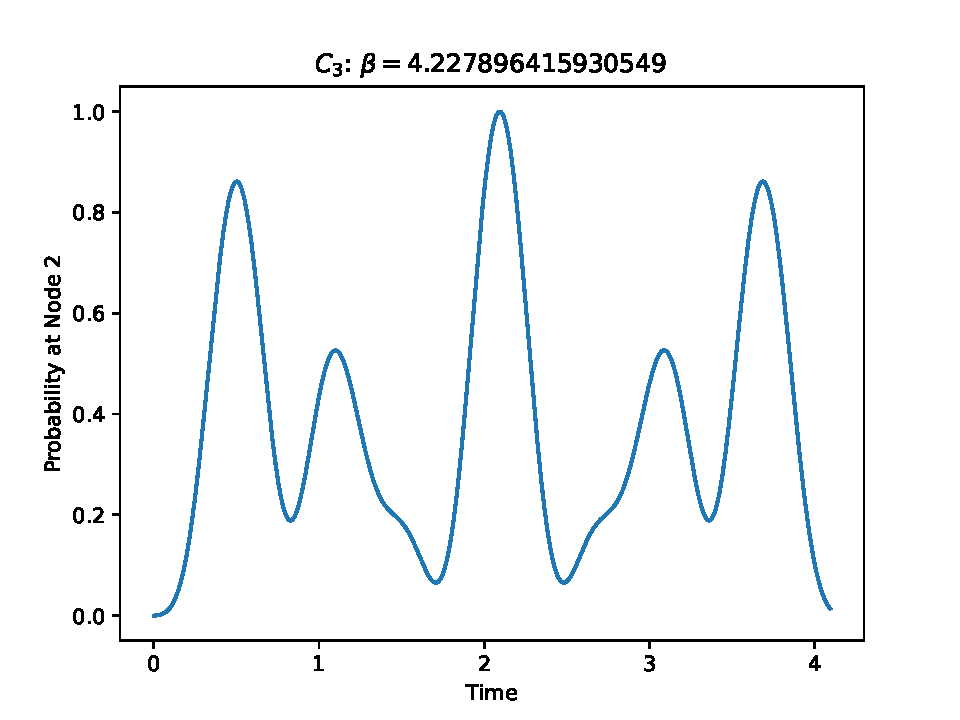
\includegraphics[width=0.49\textwidth]{c_3 (6).pdf}
    \end{figure}
    \begin{center}
        $\text{Fidelity}\geq0.999999999999$ at $t\approx\nicefrac{2\pi}{3}$
    \end{center}
\end{frame}
\begin{frame}{Is the Second Step Useless?}
    \begin{itemize}
        \item Two-step PST family can be achieved in a single step
        \item Timing of edge weight adjustment appears random, not aligned with probability peak
        \item Second step does not affect the system dynamics
    \end{itemize}
\end{frame}
\begin{frame}{C$_3$: Two-Step PST from Node 1 to Node 3}
    \begin{center}
        \begin{tikzpicture}
        % Draw nodes
        \node[circle, draw, fill=white, minimum size=1cm] (1) at (0,1.5) {1};
        \node[circle, draw, fill=white, minimum size=1cm] (2) at (2.6,-1.5) {2};
        \node[circle, draw, fill=white, minimum size=1cm] (3) at (-2.6,-1.5) {3};
        
        % Draw connections
        \draw[-] (1) -- (2) node[midway, right] {$1$};
        \draw[-] (2) -- (3) node[midway, below] {$\alpha$};
        \draw[-] (3) -- (1) node[midway, left] {$\beta$};
        
        % Labels
        \node[below] at (1) {};
        \node[below] at (2) {};
        \node[below] at (3) {};
    \end{tikzpicture}
        \begin{tikzpicture}
        % Draw nodes
        \node[circle, draw, fill=white, minimum size=1cm] (1) at (0,1.5) {1};
        \node[circle, draw, fill=white, minimum size=1cm] (2) at (2.6,-1.5) {2};
        \node[circle, draw, fill=white, minimum size=1cm] (3) at (-2.6,-1.5) {3};
        
        % Draw connections
        \draw[-] (1) -- (2) node[midway, right] {$1$};
        \draw[-] (2) -- (3) node[midway, below] {$\alpha$};
        \draw[-] (3) -- (1) node[midway, left] {$-\beta$};
        
        % Labels
        \node[below] at (1) {};
        \node[below] at (2) {};
        \node[below] at (3) {};
    \end{tikzpicture}
    \end{center}
\end{frame}
\begin{frame}{When the Second Step Matters}
    \begin{figure}
        \centering
        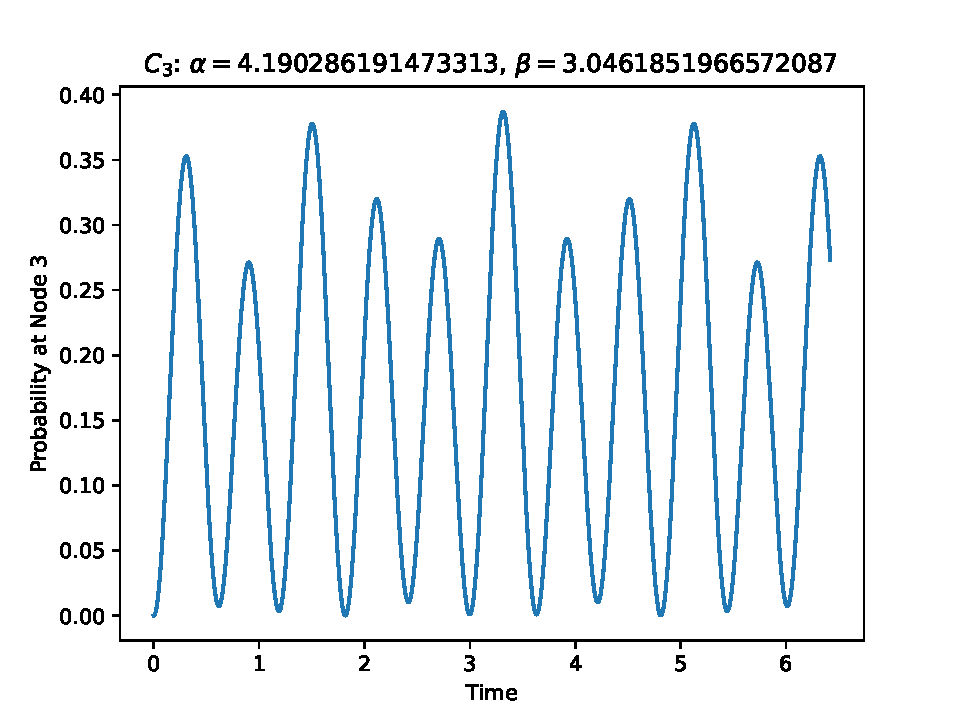
\includegraphics[width=0.59\textwidth]{c_3 (8).pdf}
    \end{figure}
\end{frame}
\begin{frame}{When the Second Step Matters}
    \begin{figure}
        \centering
        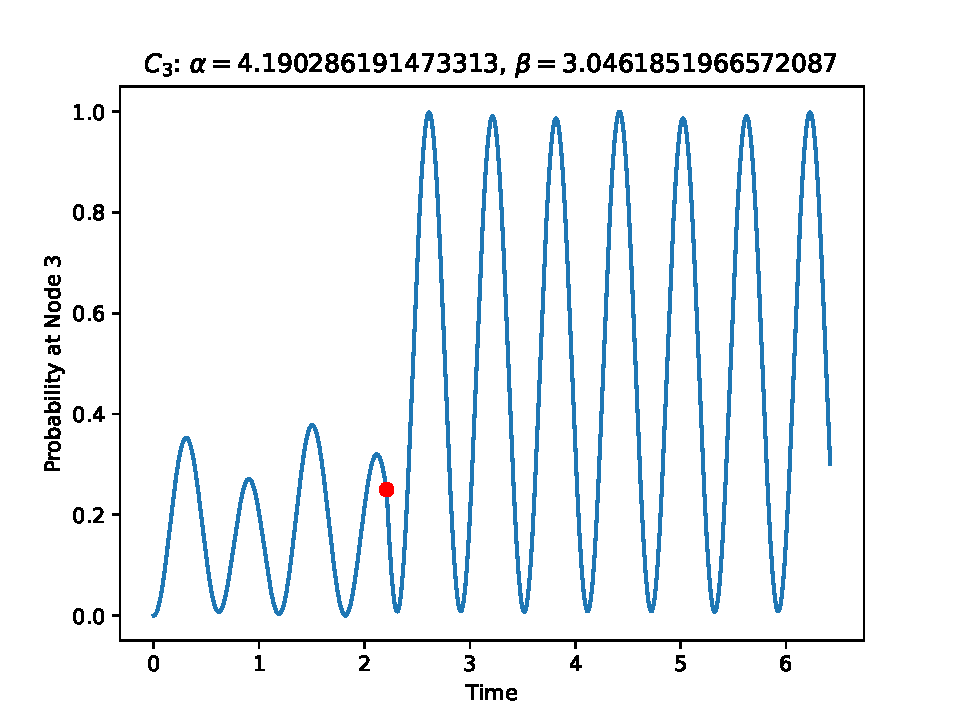
\includegraphics[width=0.59\textwidth]{c_3 (7).pdf}
    \end{figure}
    \begin{displaymath}
        \text{Fidelity}\geq0.999999999999\text{ at }t=4.420307096
    \end{displaymath}
\end{frame}
\begin{frame}{When the Second Step Matters}
    \begin{figure}
        \centering
        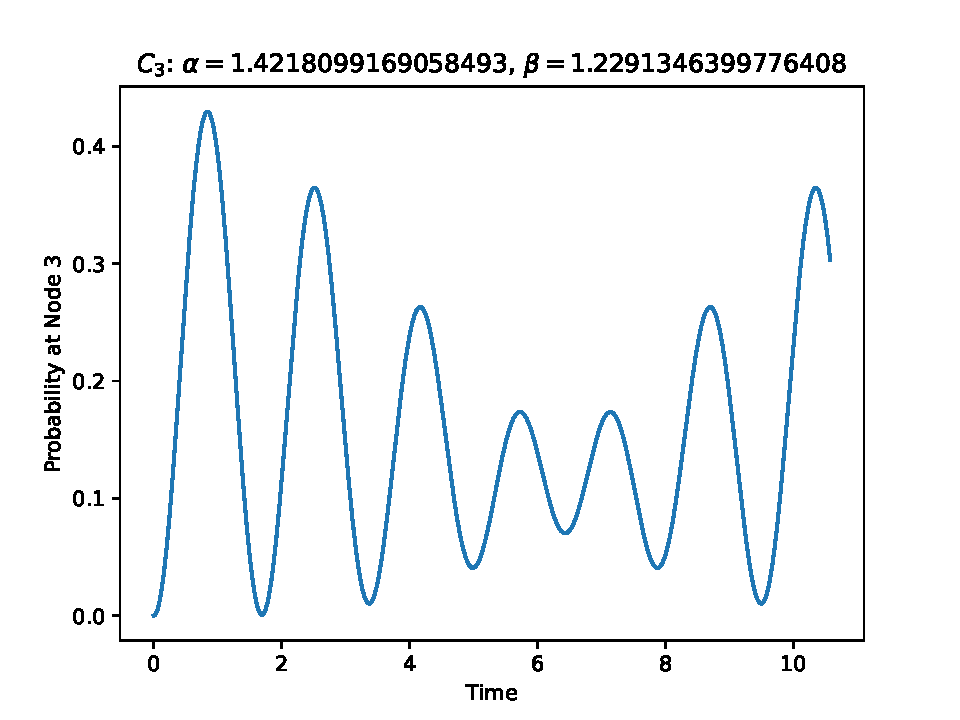
\includegraphics[width=0.59\textwidth]{c_3 (10).pdf}
    \end{figure}
\end{frame}
\begin{frame}{When the Second Step Matters}
    \begin{figure}
        \centering
        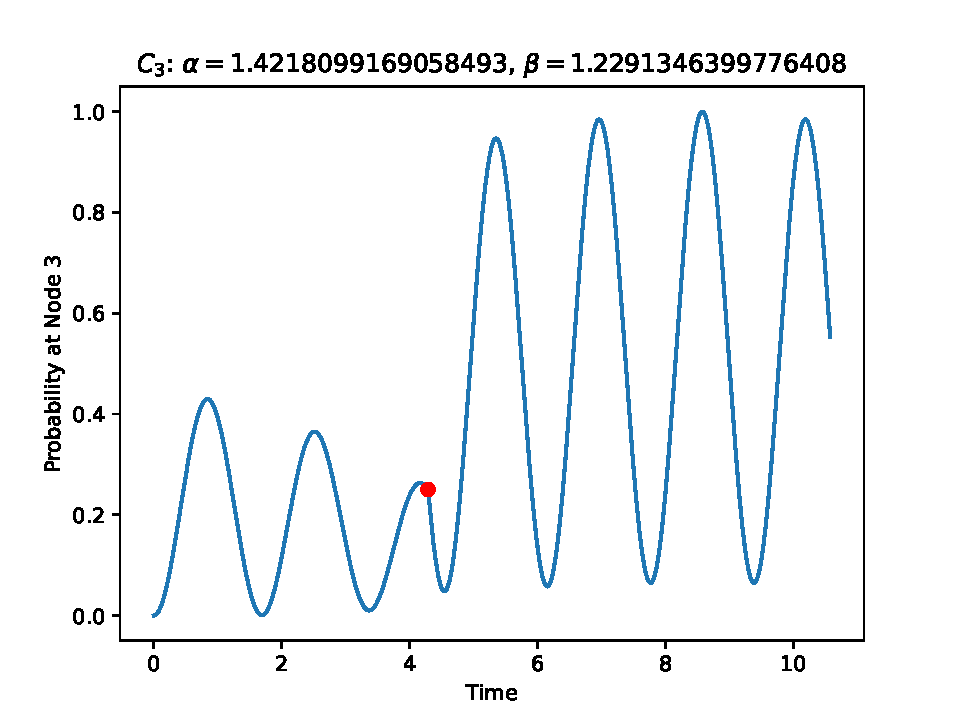
\includegraphics[width=0.59\textwidth]{c_3 (9).pdf}
    \end{figure}
    \begin{displaymath}
        \text{Fidelity}\geq0.999999999999\text{ at }t=8.576406656
    \end{displaymath}
\end{frame}
\begin{frame}{When the Second Step Matters}
    \begin{figure}
        \centering
        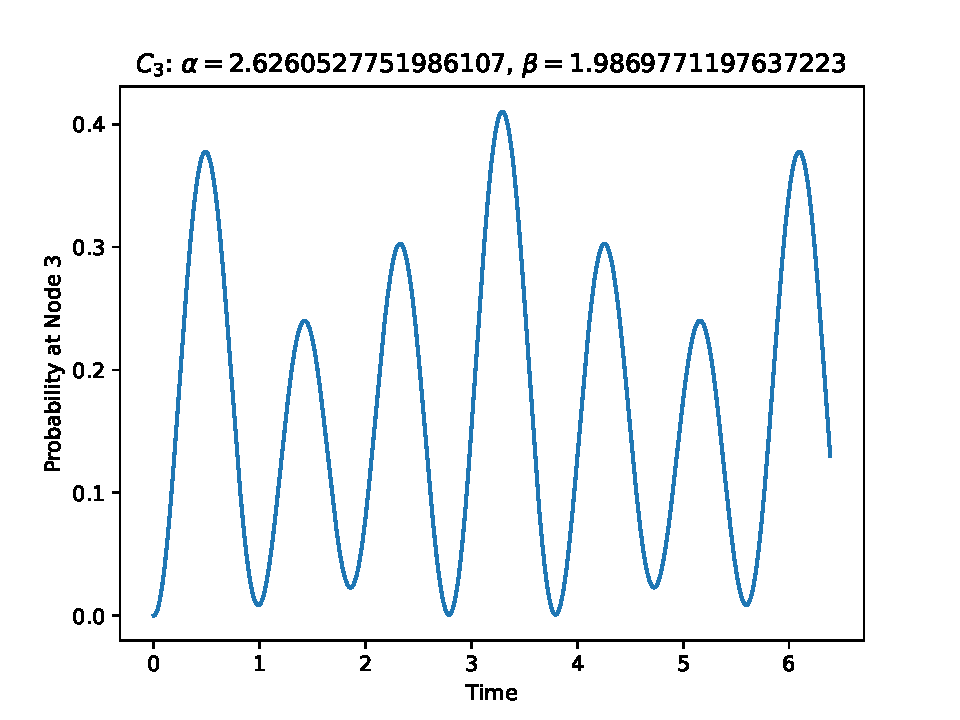
\includegraphics[width=0.59\textwidth]{c_3 (12).pdf}
    \end{figure}
\end{frame}
\begin{frame}{When the Second Step Matters}
    \begin{figure}
        \centering
        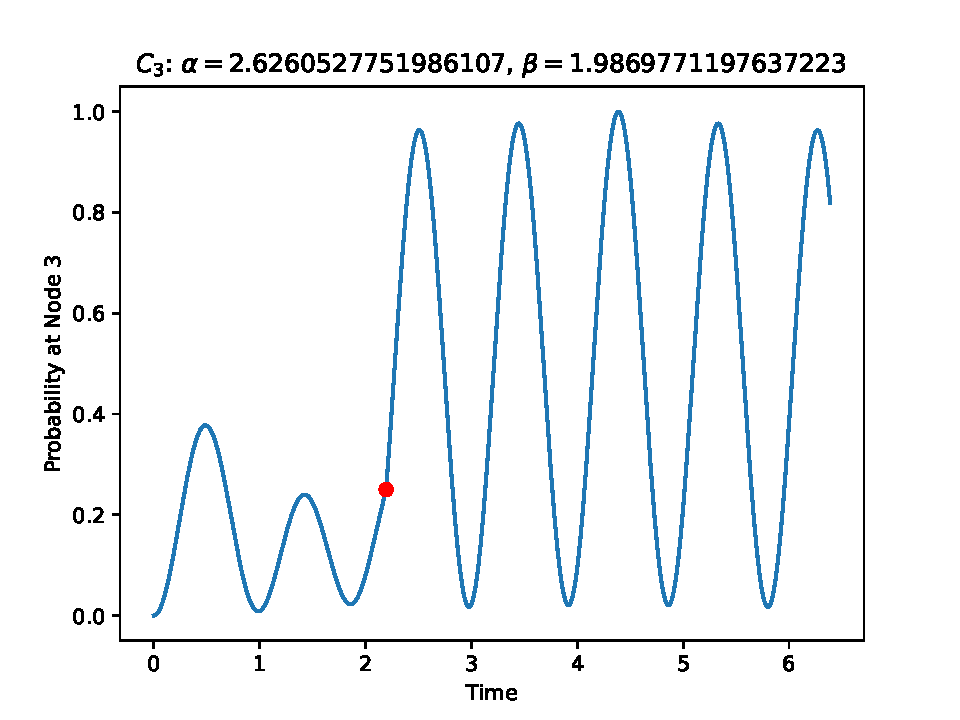
\includegraphics[width=0.59\textwidth]{c_3 (11).pdf}
    \end{figure}
    \begin{displaymath}
        \text{Fidelity}\geq0.999999999999\text{ at }t=4.38840648
    \end{displaymath}
\end{frame}
\section{Conclusion}
\begin{frame}{Conclusion}
    \begin{itemize}
        \item Extended PST on P$_4$ from two known cases to an unbounded family
        \item Real-weighted PST on C$_3$ appears likely, suggested by the $\pi$ factor in $t$, but not yet confirmed
    \end{itemize}
\end{frame}
\section{Future Directions}
\begin{frame}{Open Questions}
    \begin{itemize}
        \item Can PST on path graphs P$_n$ be characterized by a general rule?
        \item Is two-step PST the only mechanism enabling perfect fidelity on asymmetrically weighted graphs?
        \item Does allowing three-step PST reveal new or broader families?
    \end{itemize}
\end{frame}
\QApage
\end{document}
